\chapter{Implementation}
\label{chap:implementation}

\fullref{chap:methodology-requirements-system-design}{Chapter} committed the system to a latency-aware browser--server partition and closed by promising to show how that partition is realised in code, what engineering trade-offs arose, and what evidence demonstrates a working prototype. This chapter delivers the first two; the evidence is the subject of \fullref{chap:evaluation}{Chapter}. Rather than narrating every module, it is organised around the engineering problems that most shaped the prototype, each illustrated with a short extract from the codebase. The implementation was developed incrementally over roughly fifty commits, and several of the decisions below are best understood as responses to concrete failures encountered along the way.

\section{Repository and Toolchain}

The project is a single repository combining a TypeScript frontend and a Python backend. The frontend (\texttt{apps/web}) is a Vite, React, and React-Three-Fiber application responsible for audio capture, the 3D stage, and the user interface. The backend (\texttt{services/inference}) is a FastAPI WebSocket server that hosts BeatNet and Skip-BART under a conda environment with PyTorch. Two shared packages sit between them: \texttt{packages/protocol} defines the WebSocket message contract, and \texttt{packages/fixtures} defines the scene-document schema and fixture catalogue. This layout keeps the three concerns that must agree across the runtime boundary---protocol, scene model, and shared types---in one place, version-controlled together.

\section{The Protocol as a Typed Contract}
\label{sec:impl-protocol}

Requirement R4 calls for explicit, low-overhead message contracts. The implementation enforces this by making the protocol package the single authority for every message that crosses the WebSocket, defined once as a set of Zod schemas and mirrored by Pydantic models on the backend. Each message is a member of a discriminated union keyed on a \texttt{type} field, so an unknown or malformed payload is rejected at the boundary rather than fault deep in the pipeline.

\begin{lstlisting}[language=Java,caption={Downstream lighting message, defined once in the protocol package (TypeScript/Zod). The backend mirrors it in Pydantic.},label={lst:lighting-schema}]
export const lightingUpdateSchema = envelopeSchema.extend({
  type: z.literal('lighting.update'),
  hue: z.number().min(0).max(360),
  value: z.number().min(0).max(1),
  intensity: z.number().min(0).max(1).nullable(),
  // client clock of the chunk that produced this frame -> e2e latency
  originChunkTimestampMs: z.number().optional(),
  serverProcessingMs: z.number().optional(),
});
export type LightingUpdate = z.infer<typeof lightingUpdateSchema>;
\end{lstlisting}

The two diagnostic fields in \fullref{lst:lighting-schema}{Listing} are optional, which is what allowed the benchmark instrumentation of \fullref{chap:evaluation}{Chapter} to be added later without breaking compatibility with messages that predate it. The same envelope carries a protocol version, so a frontend and backend that disagree fail loudly at session initialisation instead of silently misinterpreting fields.

\section{One Audio Path for File and Microphone}
\label{sec:impl-audio}

Requirement R5 asks that file playback and microphone capture be first-class input modes, and the architecture requires them to converge before transport so that downstream processing is source-independent. Both sources feed the same Web Audio graph and are encoded into the same canonical chunk---mono, 48\,kHz, Float32 PCM, base64-encoded, and sequenced---before being sent upstream. The transport layer never learns which source produced a chunk.

One consequence of sharing a single audio graph surfaced as an audible bug: in microphone mode the speakers fed back into the input. The fix routes monitoring through an explicit gain stage that file playback re-enables and microphone capture mutes, visible in the file player's \texttt{play()} path.

\begin{lstlisting}[language=Java,caption={Restoring speaker monitoring on file playback; microphone mode mutes the same stage to prevent feedback.},label={lst:monitor}]
graph.setSource(node);
// Restore speaker output: mic mode would have muted it.
graph.setMonitor(true);
\end{lstlisting}

\section{Streaming a Model That Was Not Built to Stream}
\label{sec:impl-skipbart}

The most significant implementation challenge is that Skip-BART is not a streaming model. As discussed in \fullref{chap:theoretical-background}{Chapter}, it is autoregressive over a fixed-length input sequence and was designed to generate a lighting track for a whole piece of music in a single offline pass. The prototype, by contrast, receives audio in small chunks while the music plays. Bridging this gap is the core of the integration work, and it is done with three mechanisms.

First, the backend maintains a rolling raw-audio buffer of roughly the last ten seconds and re-runs inference over that window periodically rather than continuously. The window is bounded to keep each pass tractable, and a frame cursor ensures that only lighting frames newer than the last emitted one are published---without it, the restricted stochastic sampling would re-emit overlapping frames with different sampled colours on every pass, producing visible flicker.

\begin{lstlisting}[language=Python,caption={Sliding-window gate in the Skip-BART adapter: trim the buffer, advance the emit cursor, and only run inference once enough new audio has accumulated.},label={lst:skip-window}]
max_samples = int(WINDOW_SECONDS * self._buffer_sample_rate)
if self._buffer.size > max_samples:
    drop = self._buffer.size - max_samples
    self._buffer = self._buffer[drop:]
    self._buffer_start_ms += drop * 1000.0 / self._buffer_sample_rate
    if self._last_emitted_ms < self._buffer_start_ms:
        self._last_emitted_ms = self._buffer_start_ms

self._chunks_since_run += 1
if self._chunks_since_run < MIN_CHUNKS_BETWEEN_RUNS:
    return []          # not enough new audio yet
self._chunks_since_run = 0
\end{lstlisting}

Second, because a single window pass can take several seconds (\fullref{chap:evaluation}{Chapter} measures it at roughly eight on both test machines), running it inline would stall the chunk pipeline and freeze beat tracking. Inference therefore runs on a dedicated background worker thread: \texttt{ingest()} pushes a chunk onto a queue and returns immediately, the worker drains the queue and runs inference when the window is ready, and \texttt{get\_predictions()} non-blockingly collects whatever the worker has produced. A monotonically increasing \emph{generation} counter, checked both before processing a chunk and before publishing each predicted frame, lets a mid-stream session reset discard in-flight work without interrupting an inference already under way.

\begin{lstlisting}[language=Python,caption={Worker-thread ingest. The generation guard discards chunks enqueued before a session reset.},label={lst:skip-worker}]
def _worker_loop(self) -> None:
    while not self._stop_event.is_set():
        try:
            gen, chunk = self._in_queue.get(timeout=0.5)
        except queue.Empty:
            continue
        with self._gen_lock:
            if gen != self._generation:
                continue   # reset happened; drop stale chunk
        for pred in self._process_chunk(chunk):
            self._out_queue.put(pred)
\end{lstlisting}

Third, an early version loaded the models lazily on the first audio chunk, which produced a multi-second stall the first time playback started. Eager-loading the adapters at server startup moved that cost to launch time, where it does not affect interaction. The practical outcome of all three mechanisms is that lighting updates arrive in bursts---one burst per completed window pass---while the rest of the pipeline stays responsive. This burst behaviour is exactly what the lighting-rate measurements in \fullref{chap:evaluation}{Chapter} reflect, and it is a property of the integration strategy rather than of the transport or the worker design.

\section{Keeping the Beat Path Real-Time}
\label{sec:impl-beat}

Unlike the generative lighting path, the beat-synchronization path must stay tight to the audio, so BeatNet runs on the synchronous chunk path and was reworked to process audio per analysis hop in a streaming fashion. A second problem emerged on real music: BeatNet misses beats, and on an otherwise steady track a dropped beat visibly stalls the fixtures. The pipeline compensates with a tempo-locked phase predictor that synthesises a beat when a predicted beat time passes without a real one, while a minimum-gap filter prevents a real beat and a synthesised beat from firing within the same musical pulse. Real beats always re-anchor the predictor's phase, so synthesis fills gaps without drifting.

\begin{lstlisting}[language=Python,caption={Tempo-locked synthesis: emit a predicted beat once its time has passed, gated so it cannot land on top of a recent real beat.},label={lst:beat-synth}]
while (
    self._next_predicted_beat_ms is not None
    and self._beat_interval_ms is not None
    and self._next_predicted_beat_ms <= chunk.timestamp_ms
):
    t = self._next_predicted_beat_ms
    if t - self._last_emitted_beat_ms >= min_gap:
        envelopes.append(beat_update(beat_time_ms=t, synthetic=True))
        self._last_emitted_beat_ms = t
    self._next_predicted_beat_ms += self._beat_interval_ms
\end{lstlisting}

The \texttt{synthetic} flag travels in the beat message (\fullref{lst:lighting-schema}{Listing} shows the analogous field on lighting), so the frontend and the benchmark can distinguish real from synthesised beats; the latter counted 110--120 of roughly 130 beats per run in \fullref{chap:evaluation}{Chapter}, a direct measure of how often synthesis was doing the work.

\section{Supporting Concerns}
\label{sec:impl-supporting}

\subsection{Scene state and the runtime mapping layer}

The architecture keeps scene-document state and runtime lighting state separate but compatible. Every editor action mutates a \texttt{SceneDocument}, which the renderer draws from and which undo/redo and persistence operate on; the live lighting frame is never written into that document. Instead, a small pure function maps one lighting frame plus one fixture to the render state the 3D components consume, which is the only point at which runtime values touch the scene.

\begin{lstlisting}[language=Java,caption={The single mapping point from runtime lighting to fixture render state (TypeScript). An idle floor keeps enabled fixtures visible before the first prediction.},label={lst:map-frame}]
const value = lighting.value > 0 ? lighting.value : IDLE_VALUE_FLOOR;
const intensity = instance.enabled ? baseIntensity * value : 0;
const hue = (((lighting.hue % 360) + 360) % 360) / 360;
out.setHSL(hue, SATURATION, LIGHTNESS);
\end{lstlisting}

Keeping this mapping pure and isolated means the rendering loop can apply high-frequency lighting updates without routing them through React's reconciliation, satisfying the responsiveness rule from \fullref{sec:ch4-shared-state}{Section}.

\subsection{Robustness and observability}

Operating the prototype during development surfaced a class of failures that are invisible in offline code but routine in a live socket. Client disconnects mid-message were initially treated as errors and triggered an attempt to write to an already-closed socket; they are now treated as a clean exit. Backend stages are wrapped in lightweight timers feeding a rolling-window metrics registry---the same instrumentation later reused for the benchmark in \fullref{chap:evaluation}{Chapter}---and a structured debug log surfaces WebSocket close codes in the interface. One non-obvious transport issue is worth recording: the protocol-level WebSocket keepalive had to be disabled in development because the Vite dev proxy drops control frames, which otherwise closed the connection spuriously.

\section{The Application in Use}
\label{sec:impl-app}

\fullref{fig:impl-screenshot}{Figure} shows the running prototype. The central viewport renders the 3D stage---a truss structure carrying lighting fixtures over a reflective floor---driven live by the model output. The left panel is the fixture and structure catalogue used to compose the stage; the top bar holds audio-source selection, transport controls, and the stage import/export actions; and the right panel exposes the scene editor together with live model output and a debug log. The arrangement maps directly onto the module decomposition of \fullref{chap:methodology-requirements-system-design}{Chapter}: input and transport along the top, scene composition on the left, rendering in the centre, and shared state and diagnostics on the right.

\begin{figure}[htbp]
    \centering
    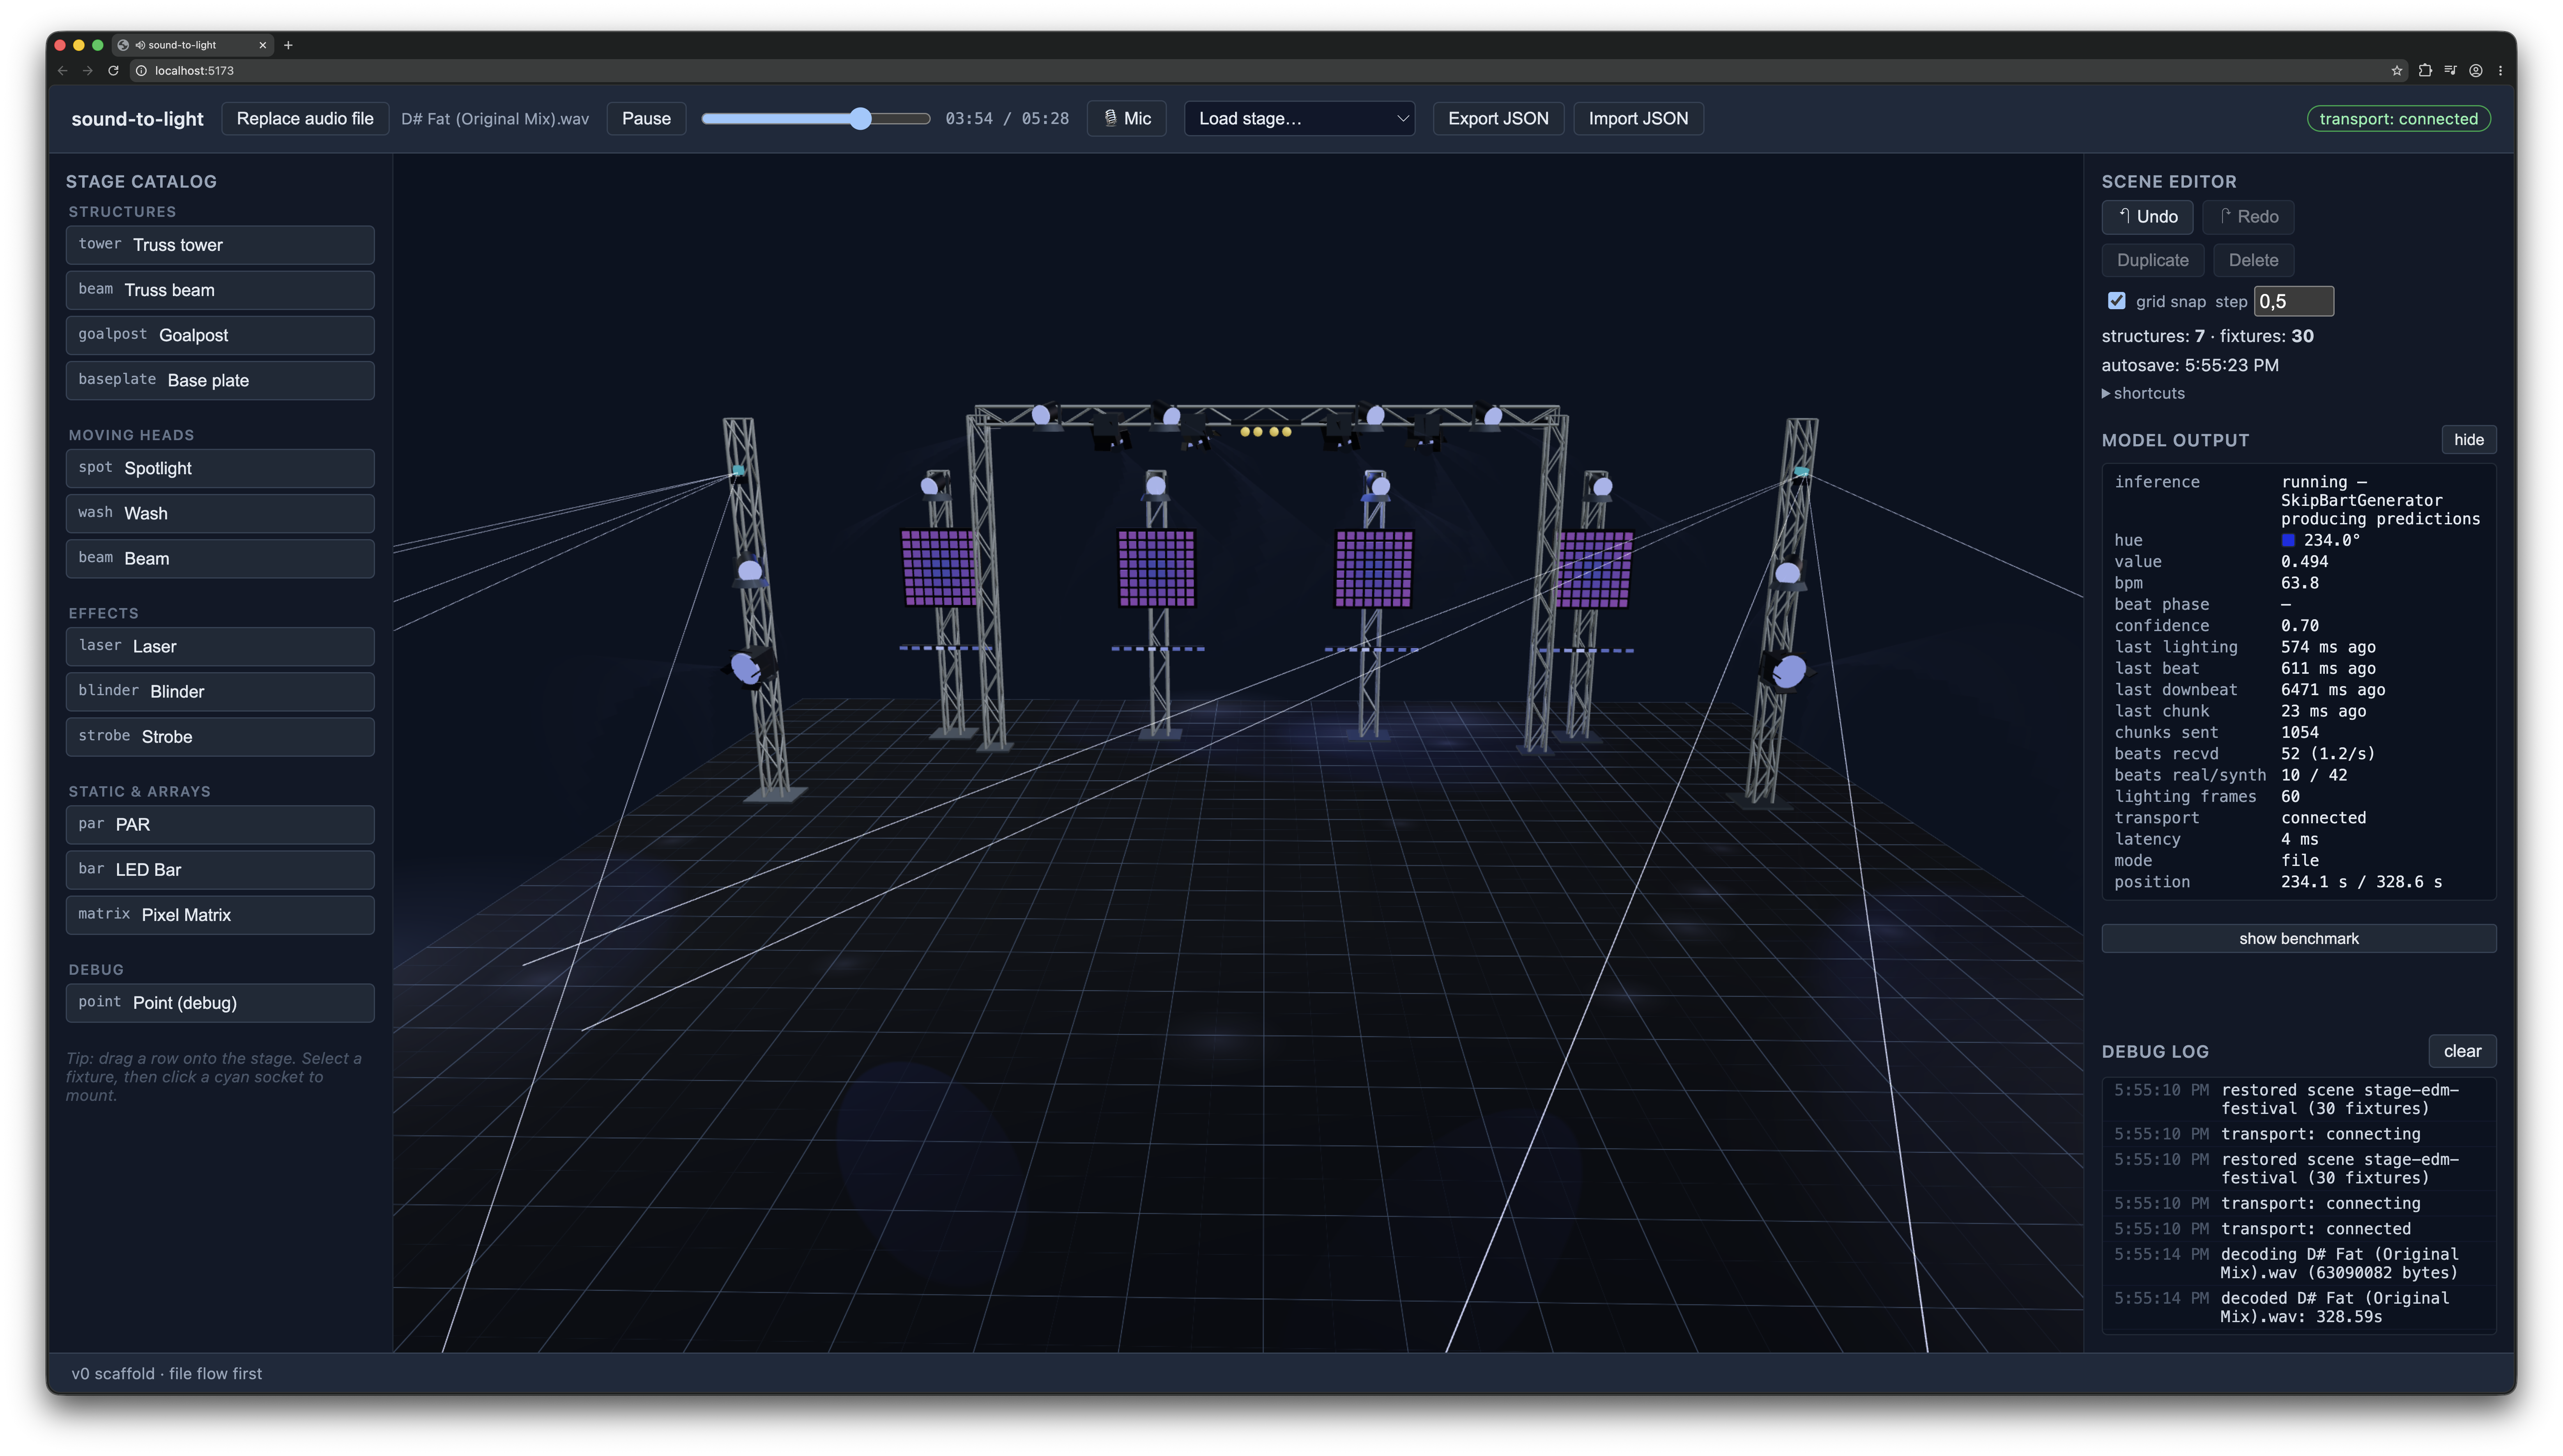
\includegraphics[width=\textwidth]{figures/chapters/5/app_screenshot.png}
    \caption{The sound-to-light prototype in use. The 3D stage (centre) is driven by live beat and lighting output from the inference server; the fixture catalogue (left), transport bar (top), and scene-editor, model-output, and debug panels (right) provide the controls and observability called for by requirements R6 and R7.}
    \label{fig:impl-screenshot}
\end{figure}

Taken together, the implementation realises the \fullref{chap:methodology-requirements-system-design}{Chapter} partition while absorbing the practical cost of running research models in a live setting: a typed protocol at the boundary, a unified audio path, an offline lighting model adapted to stream through windowing and a worker thread, a beat-synchronization path with synthesis, and a clean separation between scene state and runtime rendering. How well the resulting system performs, and where its limits lie, is quantified in \fullref{chap:evaluation}{Chapter}.
